
\begin{document}
\renewcommand{\thefigure}{SI.\arabic{figure}}
\setcounter{figure}{0}

\renewcommand{\thetable}{SI.\arabic{table}}
\setcounter{table}{0}

\section*{Supplementary Information}\label{sec:SI}

\addcontentsline{toc}{section}{Supplementary Information}
\addtocontents{toc}{\setcounter{tocdepth}{-10}}
\renewcommand{\thesubsection}{SI.\arabic{subsection}}
\setcounter{subsection}{0}


\subsection{Shannon Index and Observed OTUs plot}



\begin{figure}[H]
    \centering
    \includegraphics[scale=0.33]{./Figures/Chao_hist_empo3}
    \caption{\textbf{Distribution of Alpha Diversity in the empo\_3 samples.} A: Distribution of Chao1 index values for soil samples (4279 samples). B: Distribution of Chao1 index values for non-saline sediment samples (544 samples). C: Distribution of Chao1 index values for non-saline surface samples (1271 samples). D: Distribution of Chao1 index values for non-saline water samples (4915 samples). E: Distribution of Chao1 index values for saline sediment samples (559 samples). F: Distribution of Chao1 index values for saline surface samples (117 samples). G: Distribution of Chao1 index values for saline water samples (684 samples). H: Distribution of Chao1 index values for plant rhizosphere samples (554 samples). I: Distribution of Chao1 index values for plant surface samples (1611 samples). J: Distribution of Chao1 index values for plant corpus samples (125 samples). K: Distribution of Chao1 index values for animal secretion samples (1257 samples). L: Distribution of Chao1 index values for animal surface samples (2961 samples). M: Distribution of Chao1 index values for animal corpus samples (328 samples). N: Distribution of Chao1 index values for animal distal gut samples (4158 samples). O: Distribution of Chao1 index values for animal proximal gut samples (367 samples).}
    \label{fig:Chao_hist3}
\end{figure}

\begin{figure}[H]
    \centering
    \includegraphics[scale=0.33]{./Figures/Chao_lati_empo3}
    \caption{\textbf{The relationship between Chao1 index and latitude.} A: Trend of Chao1 index with latitude for soil samples. B: Trend of Chao1 index with latitude for non-saline water (water and sediment) samples. C: Trend of Chao1 index with latitude for saline water (water and sediment) samples. D: Trend of Chao1 index with latitude for non-saline sediment samples. E: Trend of Chao1 index with latitude for non-saline surface samples. F: Trend of Chao1 index with latitude for non-saline water samples. G: Trend of Chao1 index with latitude for saline sediment samples. H: Trend of Chao1 index with latitude for saline surface samples. I: Trend of Chao1 index with latitude for saline water samples. J: Trend of Chao1 index with latitude for animal surface samples. K: Trend of Chao1 index with latitude for plant surface samples. L: Trend of Chao1 index with latitude for plant rhizosphere samples.}
    \label{fig:Chao_lati3}
\end{figure}

\begin{figure}[H]
    \centering
    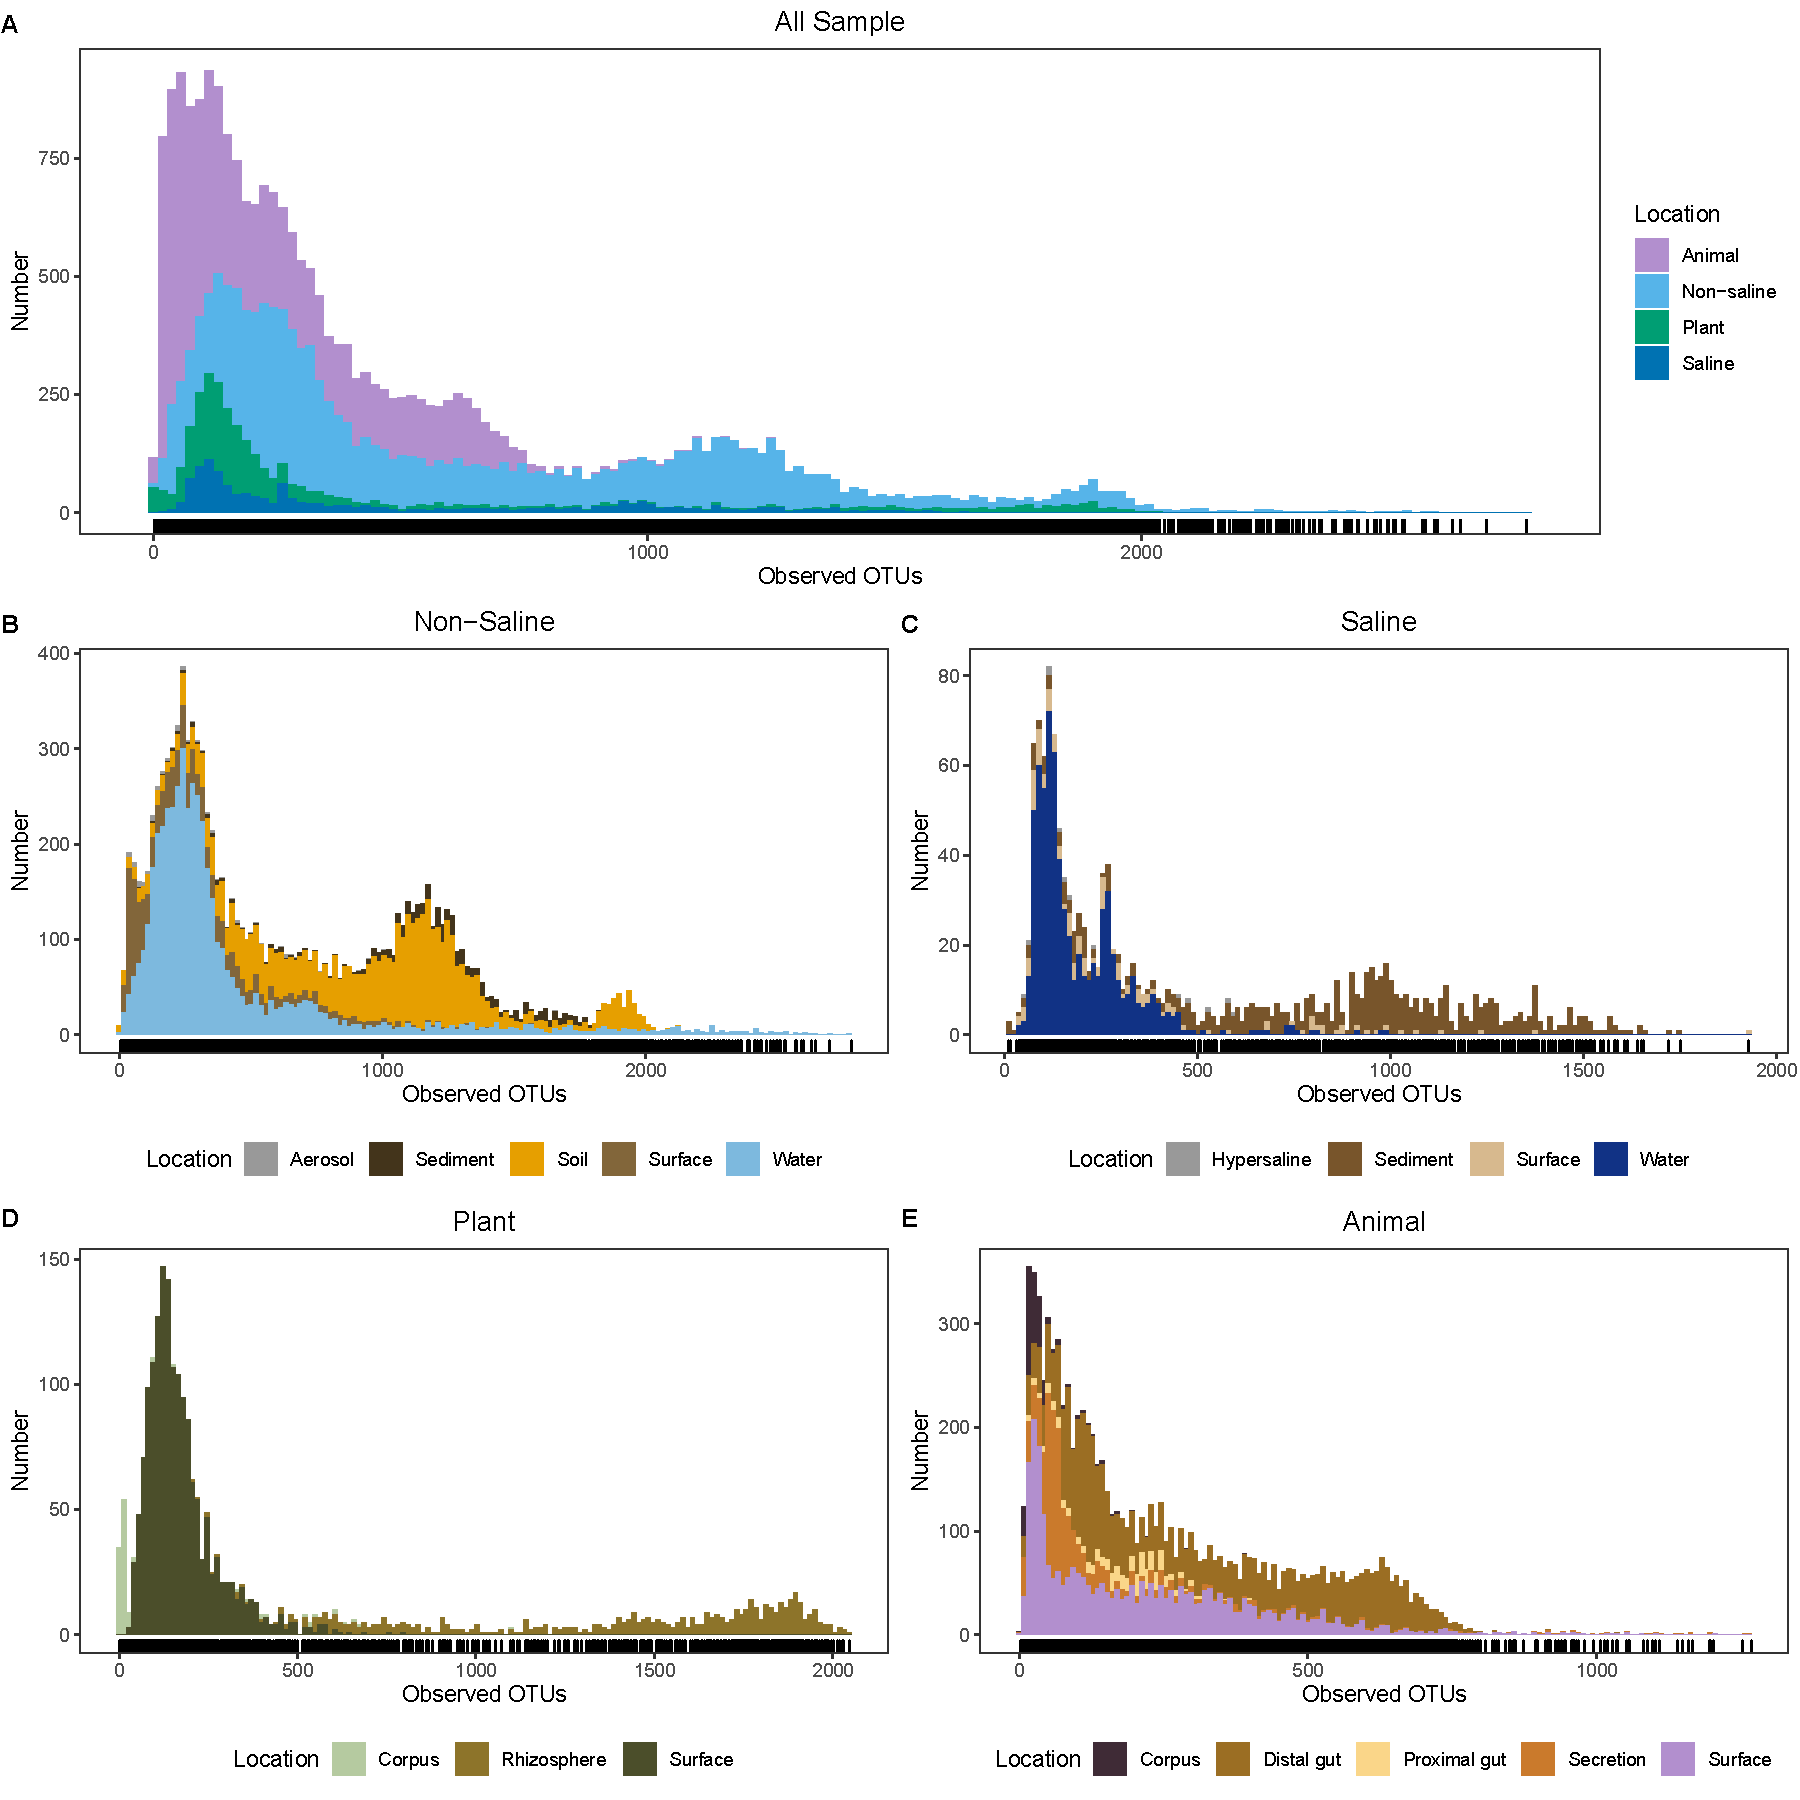
\includegraphics[scale=0.33]{./Figures/OO_hist_empo2}
    \caption{\textbf{Distribution of Observed OTUs in the whole dataset.} A: Distribution of Observed OTUs in the total dataset (23,820 samples, bin=150). B: Distribution of Observed OTUs for non-saline samples (11094 samples, bin=150). C: Distribution of Observed OTUs for saline samples (1373 samples, bin=150). D: Distribution of Observed OTUs for plant samples (2290 samples, bin=150). E: Distribution of Observed OTUs for animal samples (9071 samples, bin=150).}
    \label{fig:OO_hist}
\end{figure}

\begin{figure}[H]
    \centering
    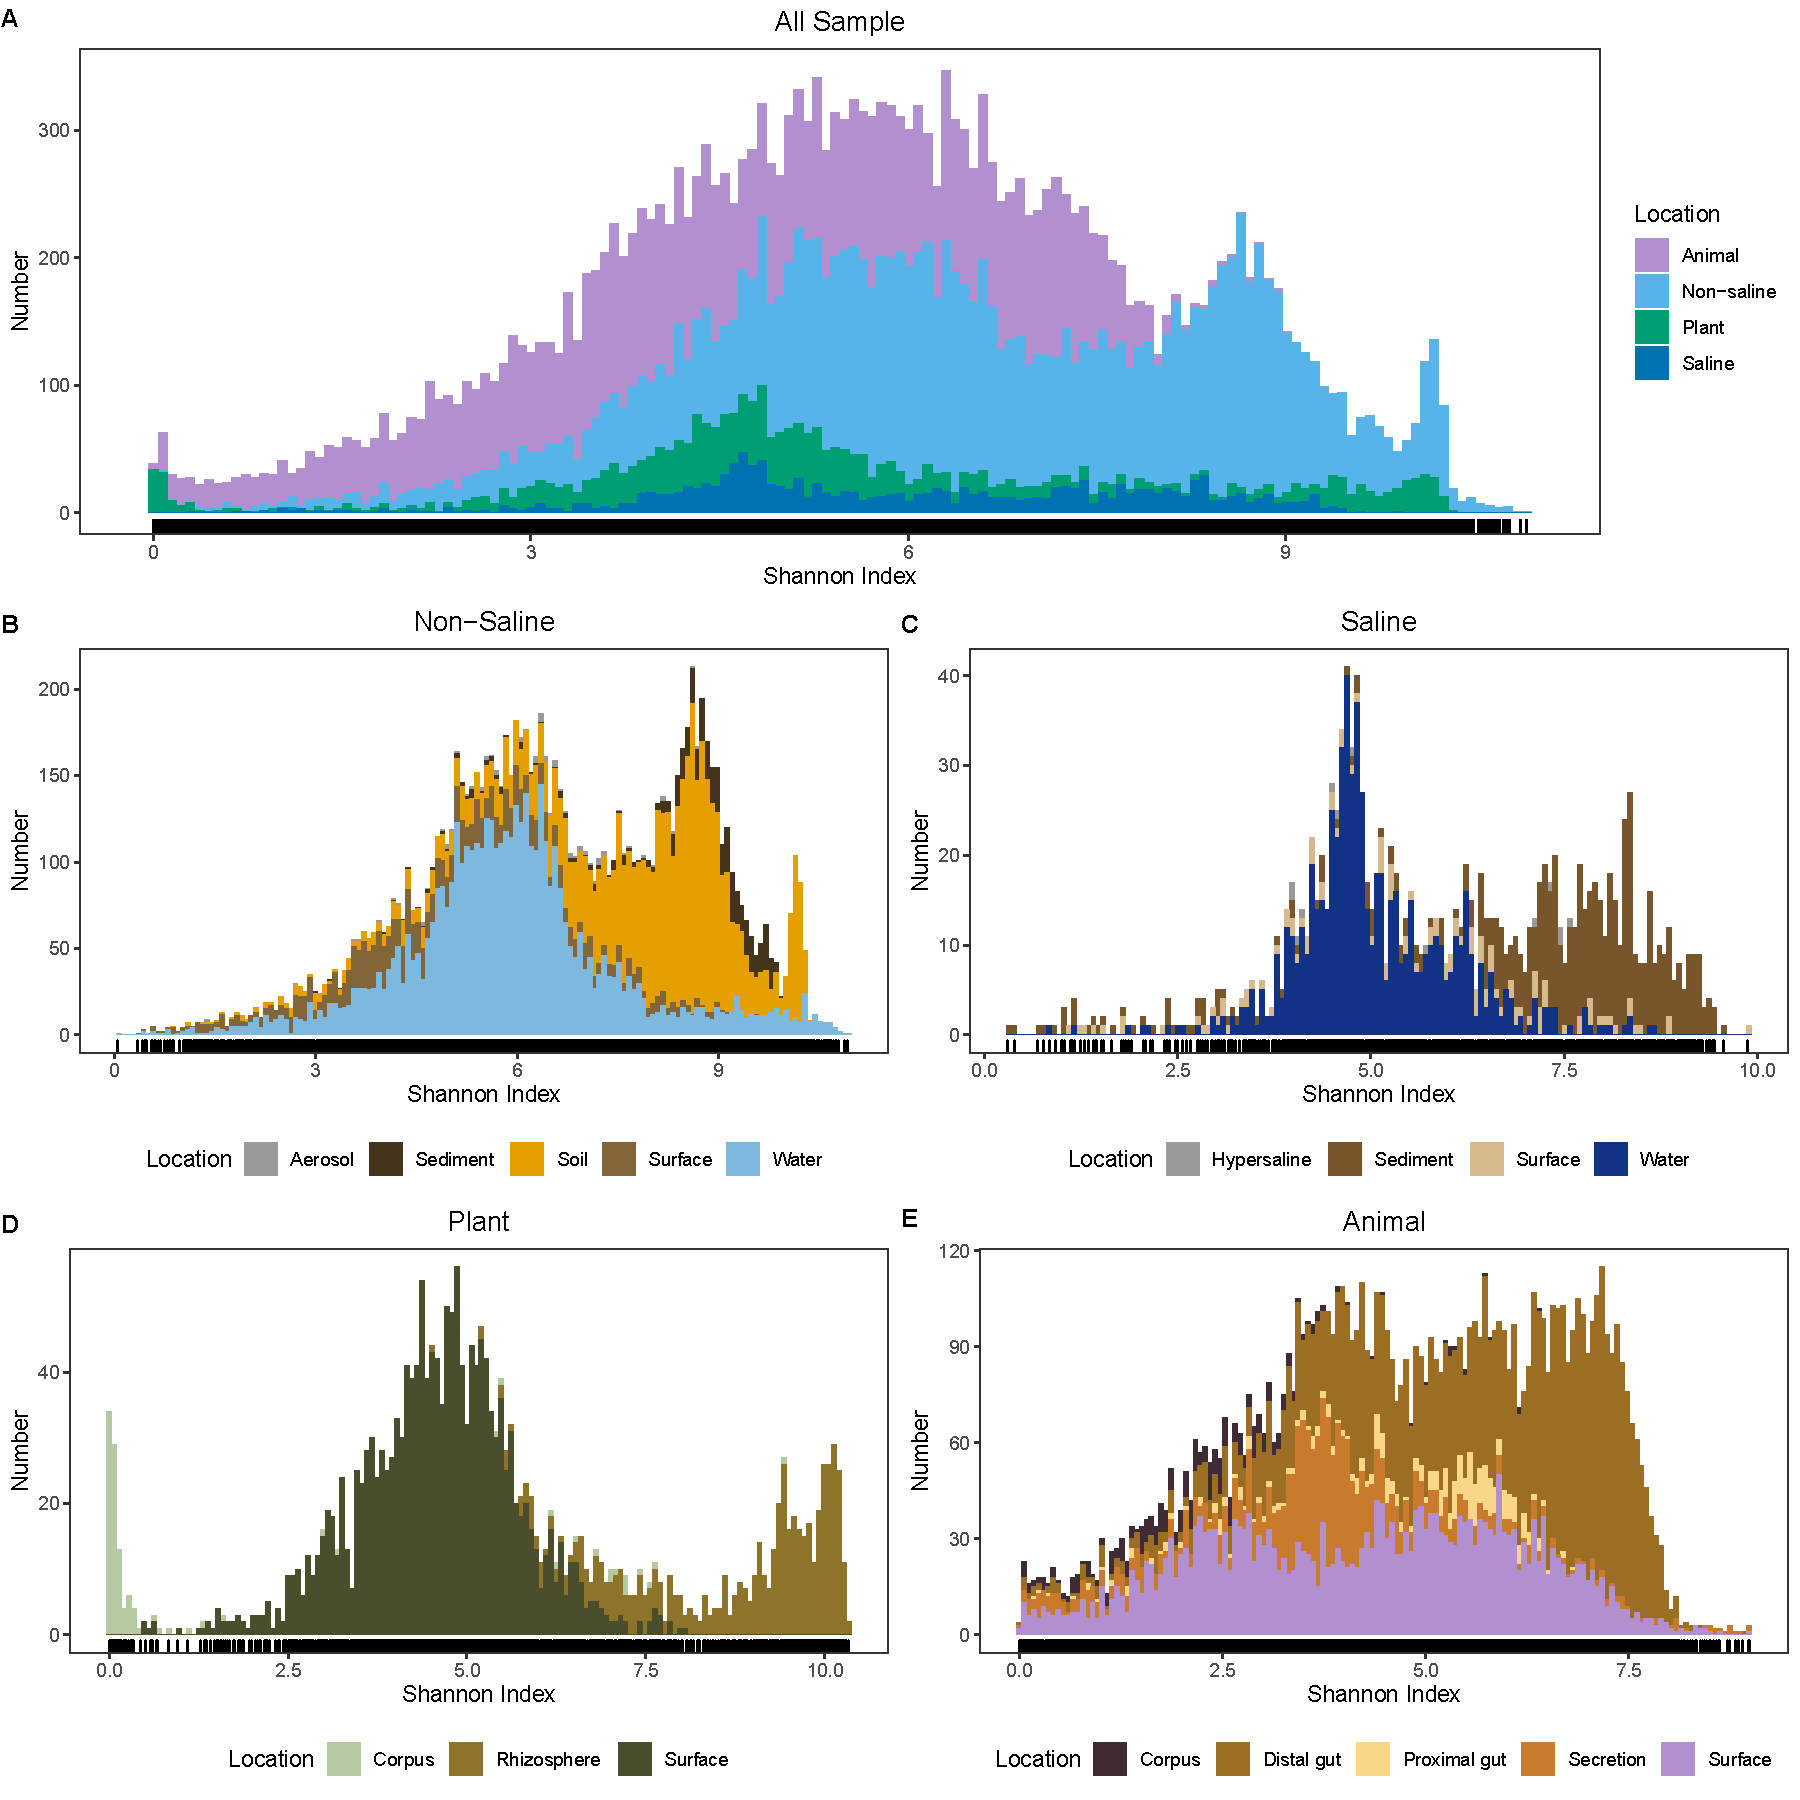
\includegraphics[scale=0.33]{./Figures/Shan_hist_empo2}
    \caption{\textbf{Distribution of Shannon index in the whole dataset.} A: Distribution of Shannon index values in the total dataset (23,820 samples, bin=150). B: Distribution of Shannon index values for non-saline samples (11094 samples, bin=150). C: Distribution of Shannon index values for saline samples (1373 samples, bin=150). D: Distribution of Shannon index values for plant samples (2290 samples, bin=150). E: Distribution of Shannon index values for animal samples (9071 samples, bin=150).}
    \label{fig:Shan_hist}
\end{figure}

\begin{figure}[H]
    \centering
    \includegraphics[scale=0.33]{./Figures/OO_hist_empo3}
    \caption{\textbf{Distribution of observed OTUs in the empo\_3 samples.} A: Distribution of observed OTUs for soil samples (4279 samples). B: Distribution of observed OTUs for non-saline sediment samples (544 samples). C: Distribution of observed OTUs for non-saline surface samples (1271 samples). D: Distribution of observed OTUs for non-saline water samples (4915 samples). E: Distribution of observed OTUs for saline sediment samples (559 samples). F: Distribution of observed OTUs for saline surface samples (117 samples). G: Distribution of observed OTUs for saline water samples (684 samples). H: Distribution of observed OTUs for plant rhizosphere samples (554 samples). I: Distribution of observed OTUs for plant surface samples (1611 samples). J: Distribution of observed OTUs for plant corpus samples (125 samples). K: Distribution of observed OTUs for animal secretion samples (1257 samples). L: Distribution of observed OTUs for animal surface samples (2961 samples). M: Distribution of observed OTUs for animal corpus samples (328 samples). N: Distribution of observed OTUs for animal distal gut samples (4158 samples). O: Distribution of observed OTUs for animal proximal gut samples (367 samples).}
    \label{fig:OO_hist3}
\end{figure}

\begin{figure}[H]
    \centering
    \includegraphics[scale=0.33]{./Figures/Shan_hist_empo3}
    \caption{\textbf{Distribution of Shannon index in the empo\_3 samples.} A: Distribution of Shannon index values for soil samples (4279 samples). B: Distribution of Shannon index values for non-saline sediment samples (544 samples). C: Distribution of Shannon index values for non-saline surface samples (1271 samples). D: Distribution of Shannon index values for non-saline water samples (4915 samples). E: Distribution of Shannon index values for saline sediment samples (559 samples). F: Distribution of Shannon index values for saline surface samples (117 samples). G: Distribution of Shannon index values for saline water samples (684 samples). H: Distribution of Shannon index values for plant rhizosphere samples (554 samples). I: Distribution of Shannon index values for plant surface samples (1611 samples). J: Distribution of Shannon index values for plant corpus samples (125 samples). K: Distribution of Shannon index values for animal secretion samples (1257 samples). L: Distribution of Shannon index values for animal surface samples (2961 samples). M: Distribution of Shannon index values for animal corpus samples (328 samples). N: Distribution of Shannon index values for animal distal gut samples (4158 samples). O: Distribution of Shannon index values for animal proximal gut samples (367 samples).}
    \label{fig:Shan_hist3}
\end{figure}

\begin{figure}[H]
    \centering
    \includegraphics[scale=0.33]{./Figures/OO_T_empo2}
    \caption{\textbf{The relationship between observed OTUs and temperature.} A: Trend of observed OTUs with temperature for samples in the whole dataset. B: Trend of observed OTUs with temperature for non-saline samples. C: Trend of observed OTUs with temperature for saline samples. D: Trend of observed OTUs with temperature for plant samples.}
    \label{fig:OO_T}
\end{figure}

\begin{figure}[H]
    \centering
    \includegraphics[scale=0.33]{./Figures/Shan_T_empo2}
    \caption{\textbf{The relationship between Shannon index and temperature.} A: Trend of Shannon index with temperature for samples in the whole dataset. B: Trend of Shannon index with temperature for non-saline samples. C: Trend of Shannon index with temperature for saline samples. D: Trend of Shannon index with temperature for plant samples.}
    \label{fig:Shan_T}
\end{figure}


\begin{figure}[H]
    \centering
    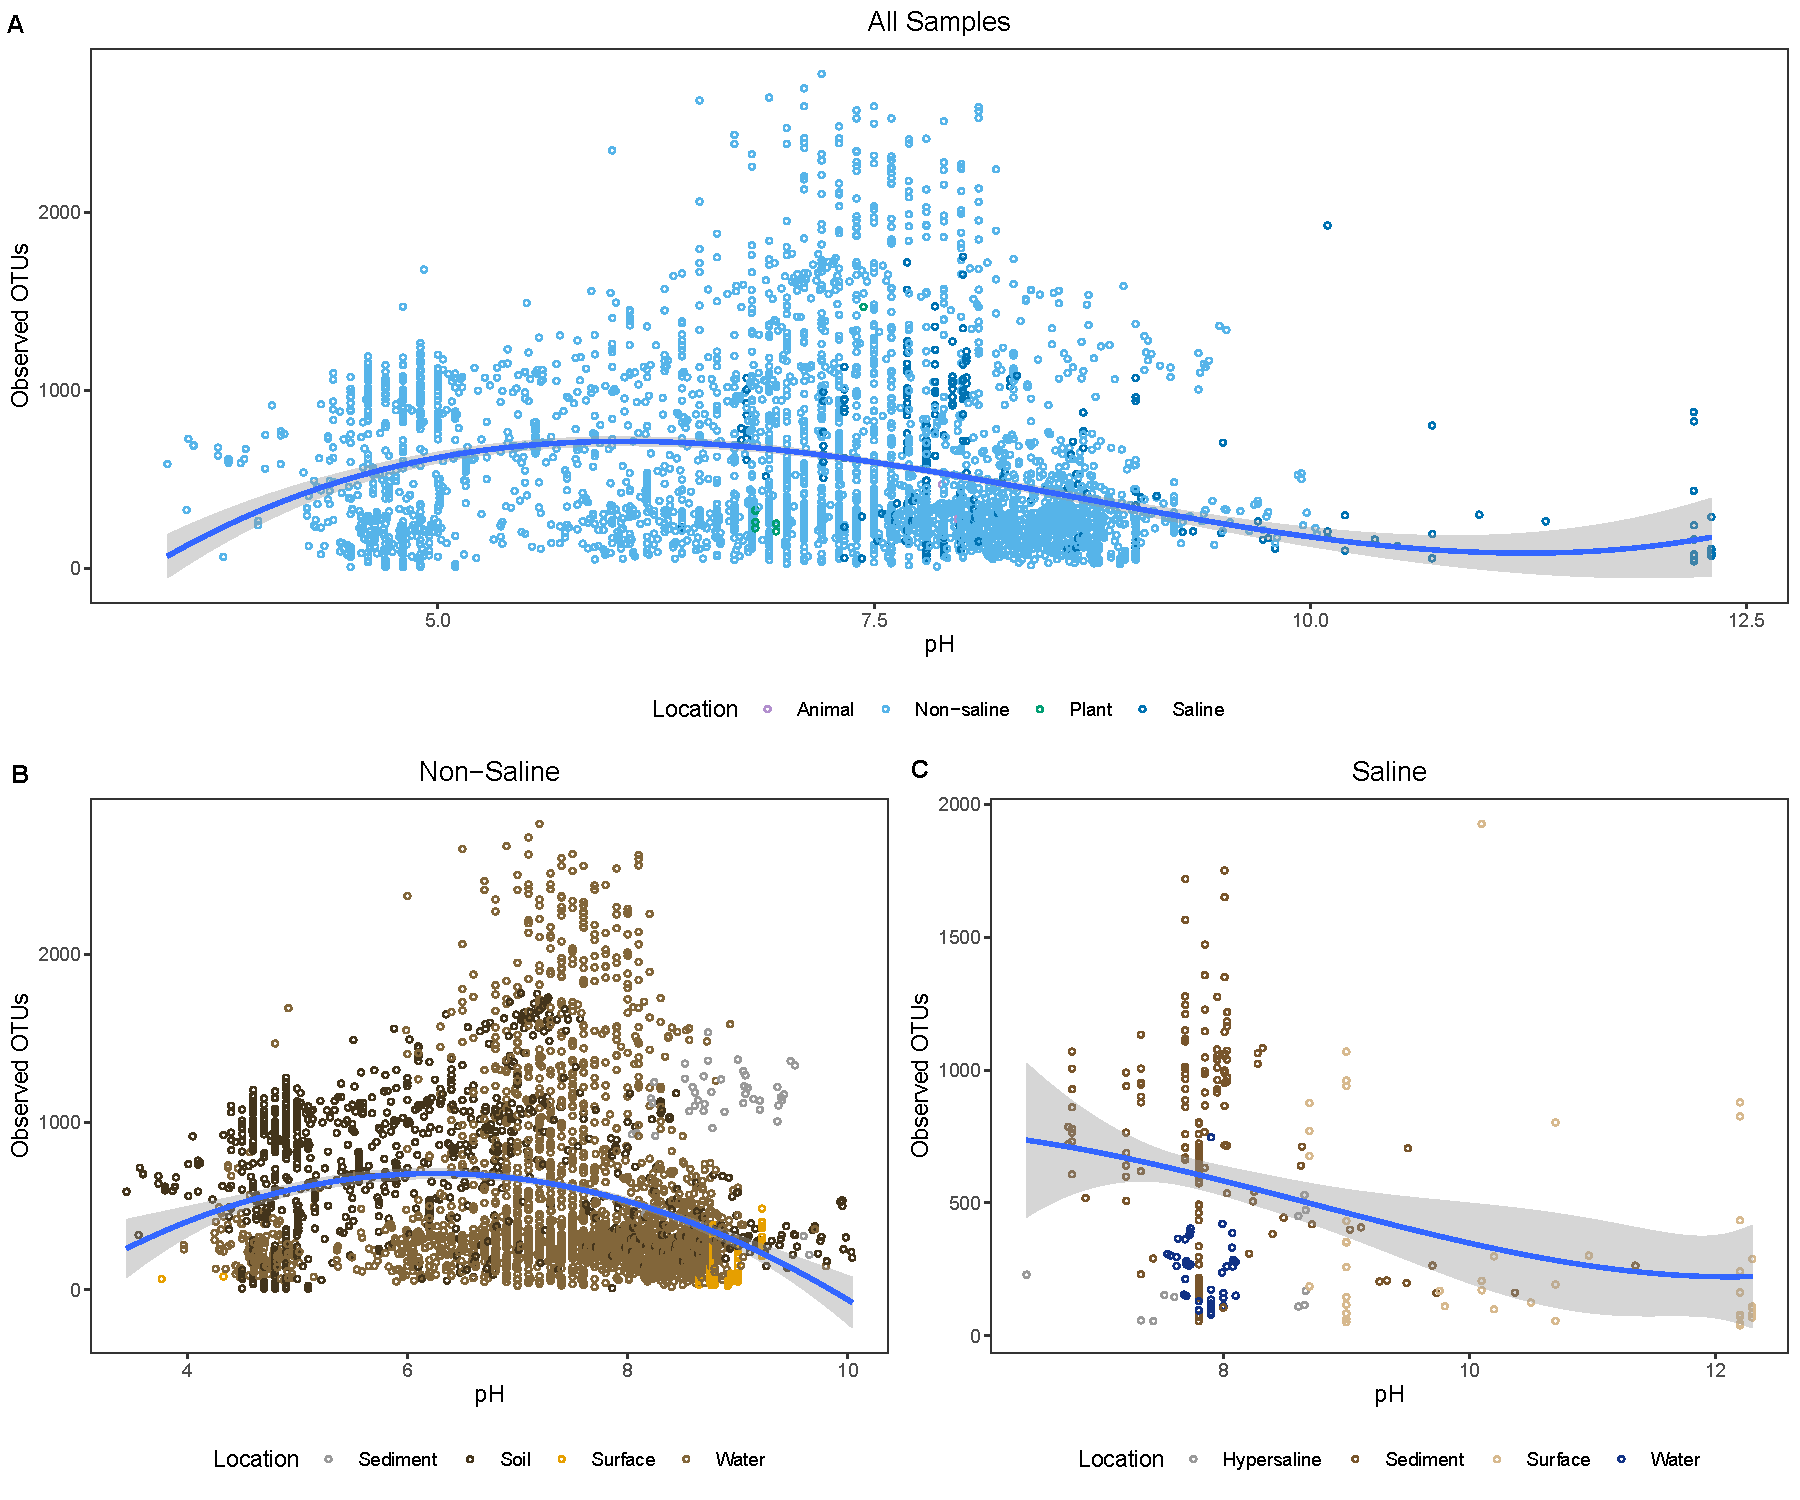
\includegraphics[scale=0.33]{./Figures/OO_pH_empo2}
    \caption{\textbf{The relationship between observed OTUs and pH.} A: Trend of observed OTUs with pH for samples in the whole dataset. B: Trend of observed OTUs with pH for non-saline samples. C: Trend of observed OTUs with pH for saline samples.}
    \label{fig:OO_pH}
\end{figure}

\begin{figure}[H]
    \centering
    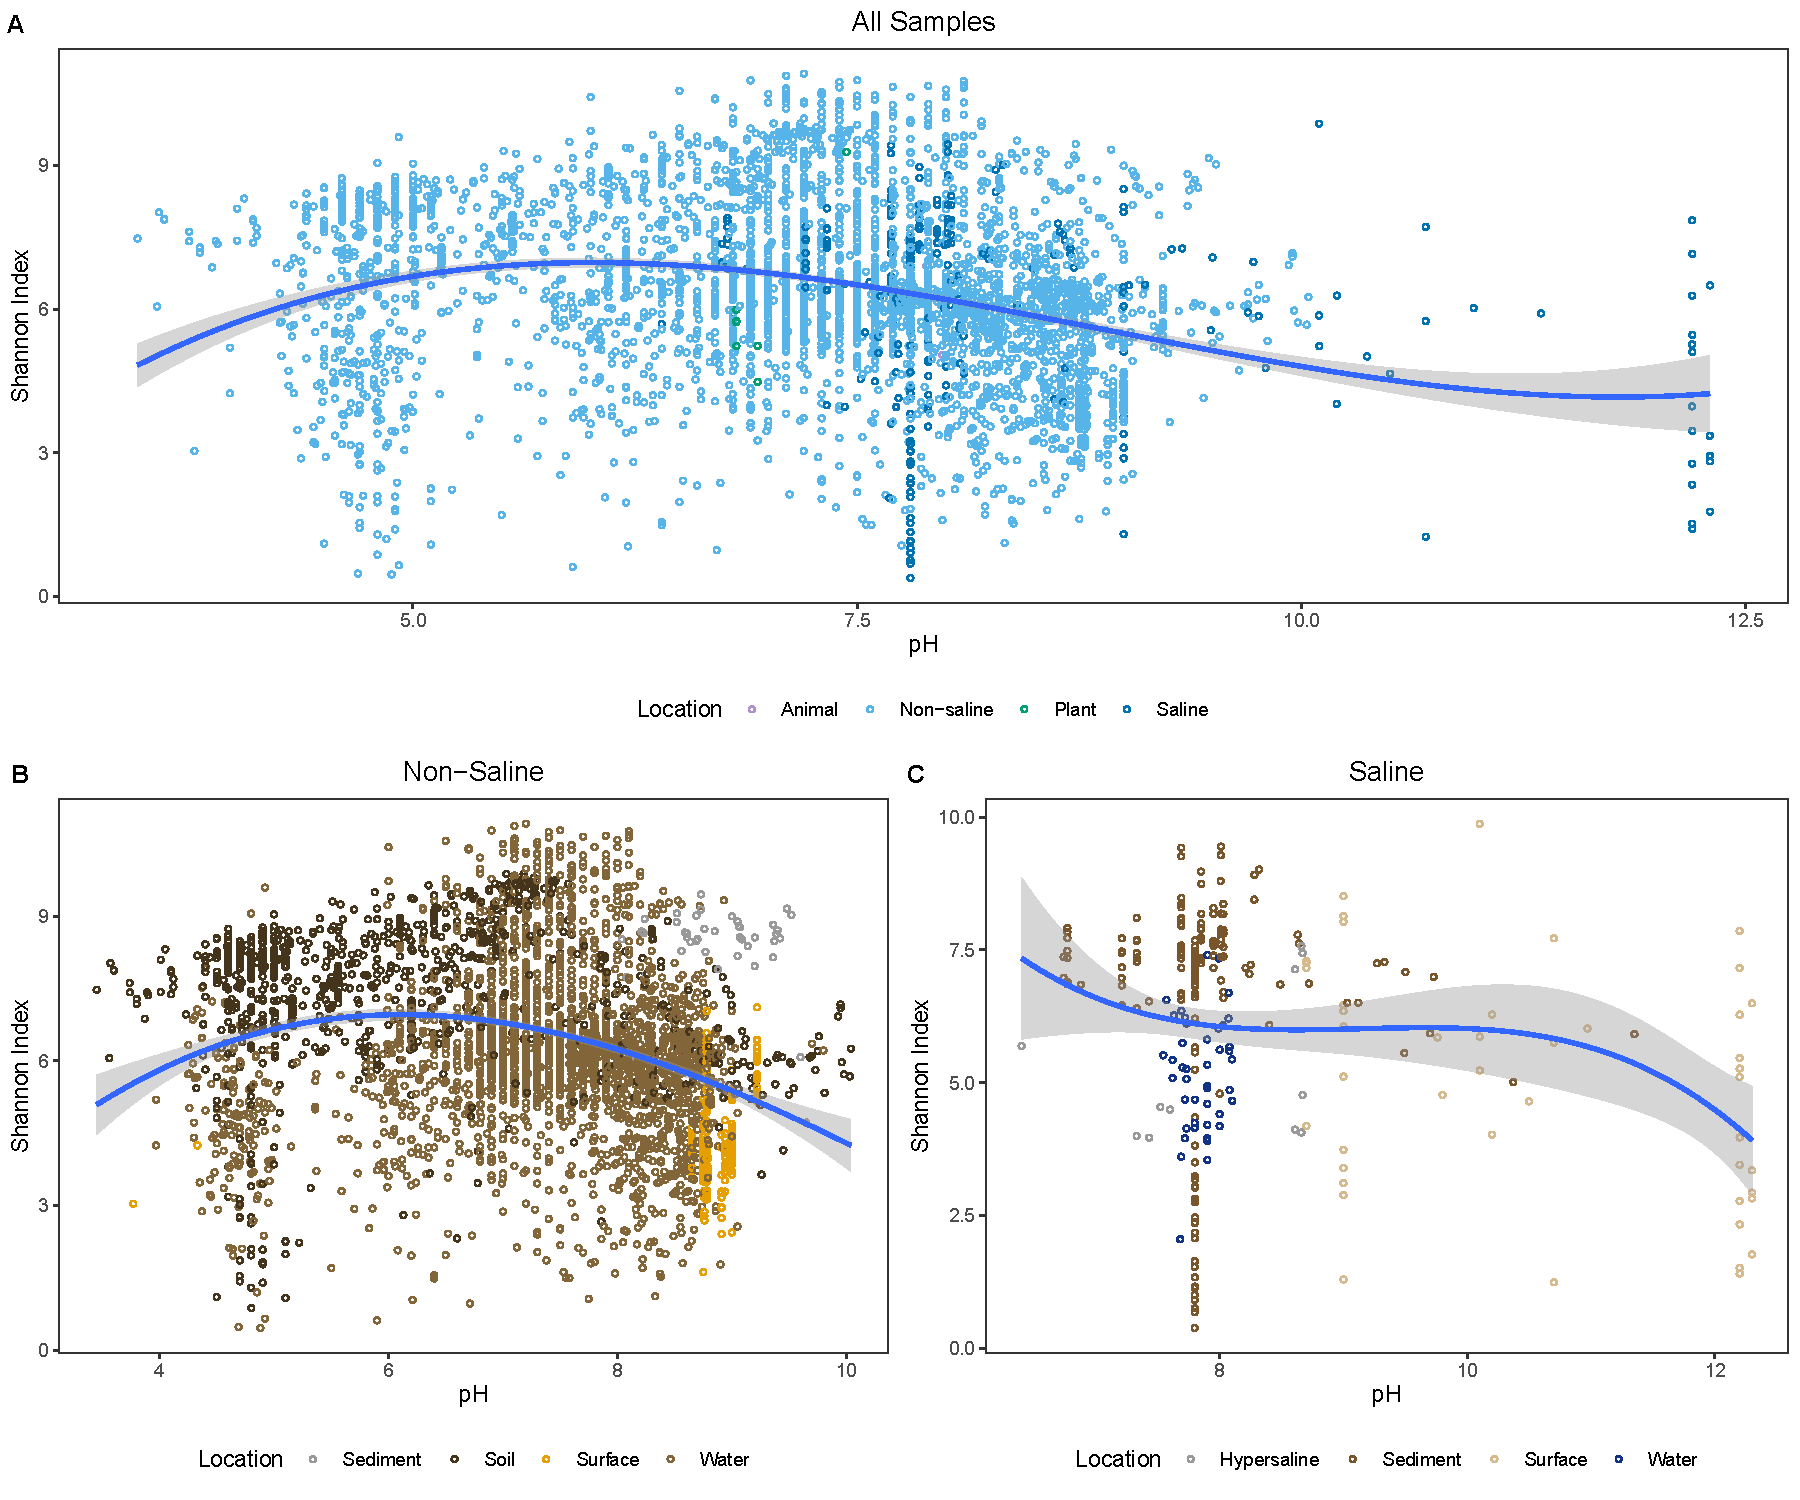
\includegraphics[scale=0.33]{./Figures/Shan_pH_empo2}
    \caption{\textbf{The relationship between Shannon index and pH.} A: Trend of Shannon index with pH for samples in the whole dataset. B: Trend of Shannon index with pH for non-saline samples. C: Trend of Shannon index with pH for saline samples.}
    \label{fig:Shan_pH}
\end{figure}

\begin{figure}[H]
    \centering
    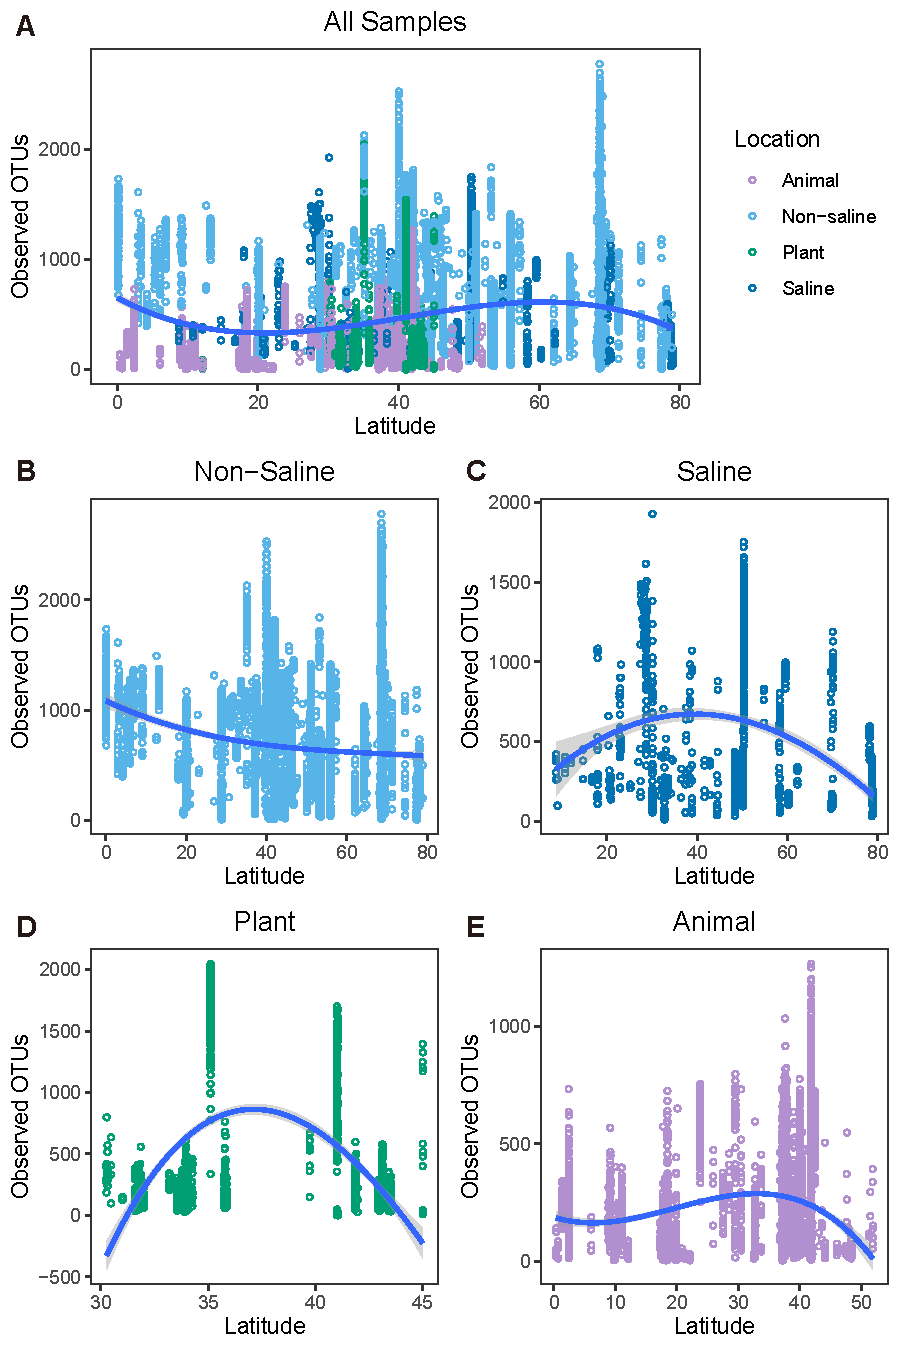
\includegraphics[scale=0.33]{./Figures/OO_lati_empo2}
    \caption{\textbf{The relationship between observed OTUs and latitude.} A: Trend of observed OTUs with latitude for samples in the whole dataset. B: Trend of observed OTUs with latitude for non-saline samples. C: Trend of observed OTUs with latitude for saline samples. D: Trend of observed OTUs with latitude for plant samples. E: Trend of observed OTUs with latitude for animal samples.}
    \label{fig:OO_lati}
\end{figure}

\begin{figure}[H]
    \centering
    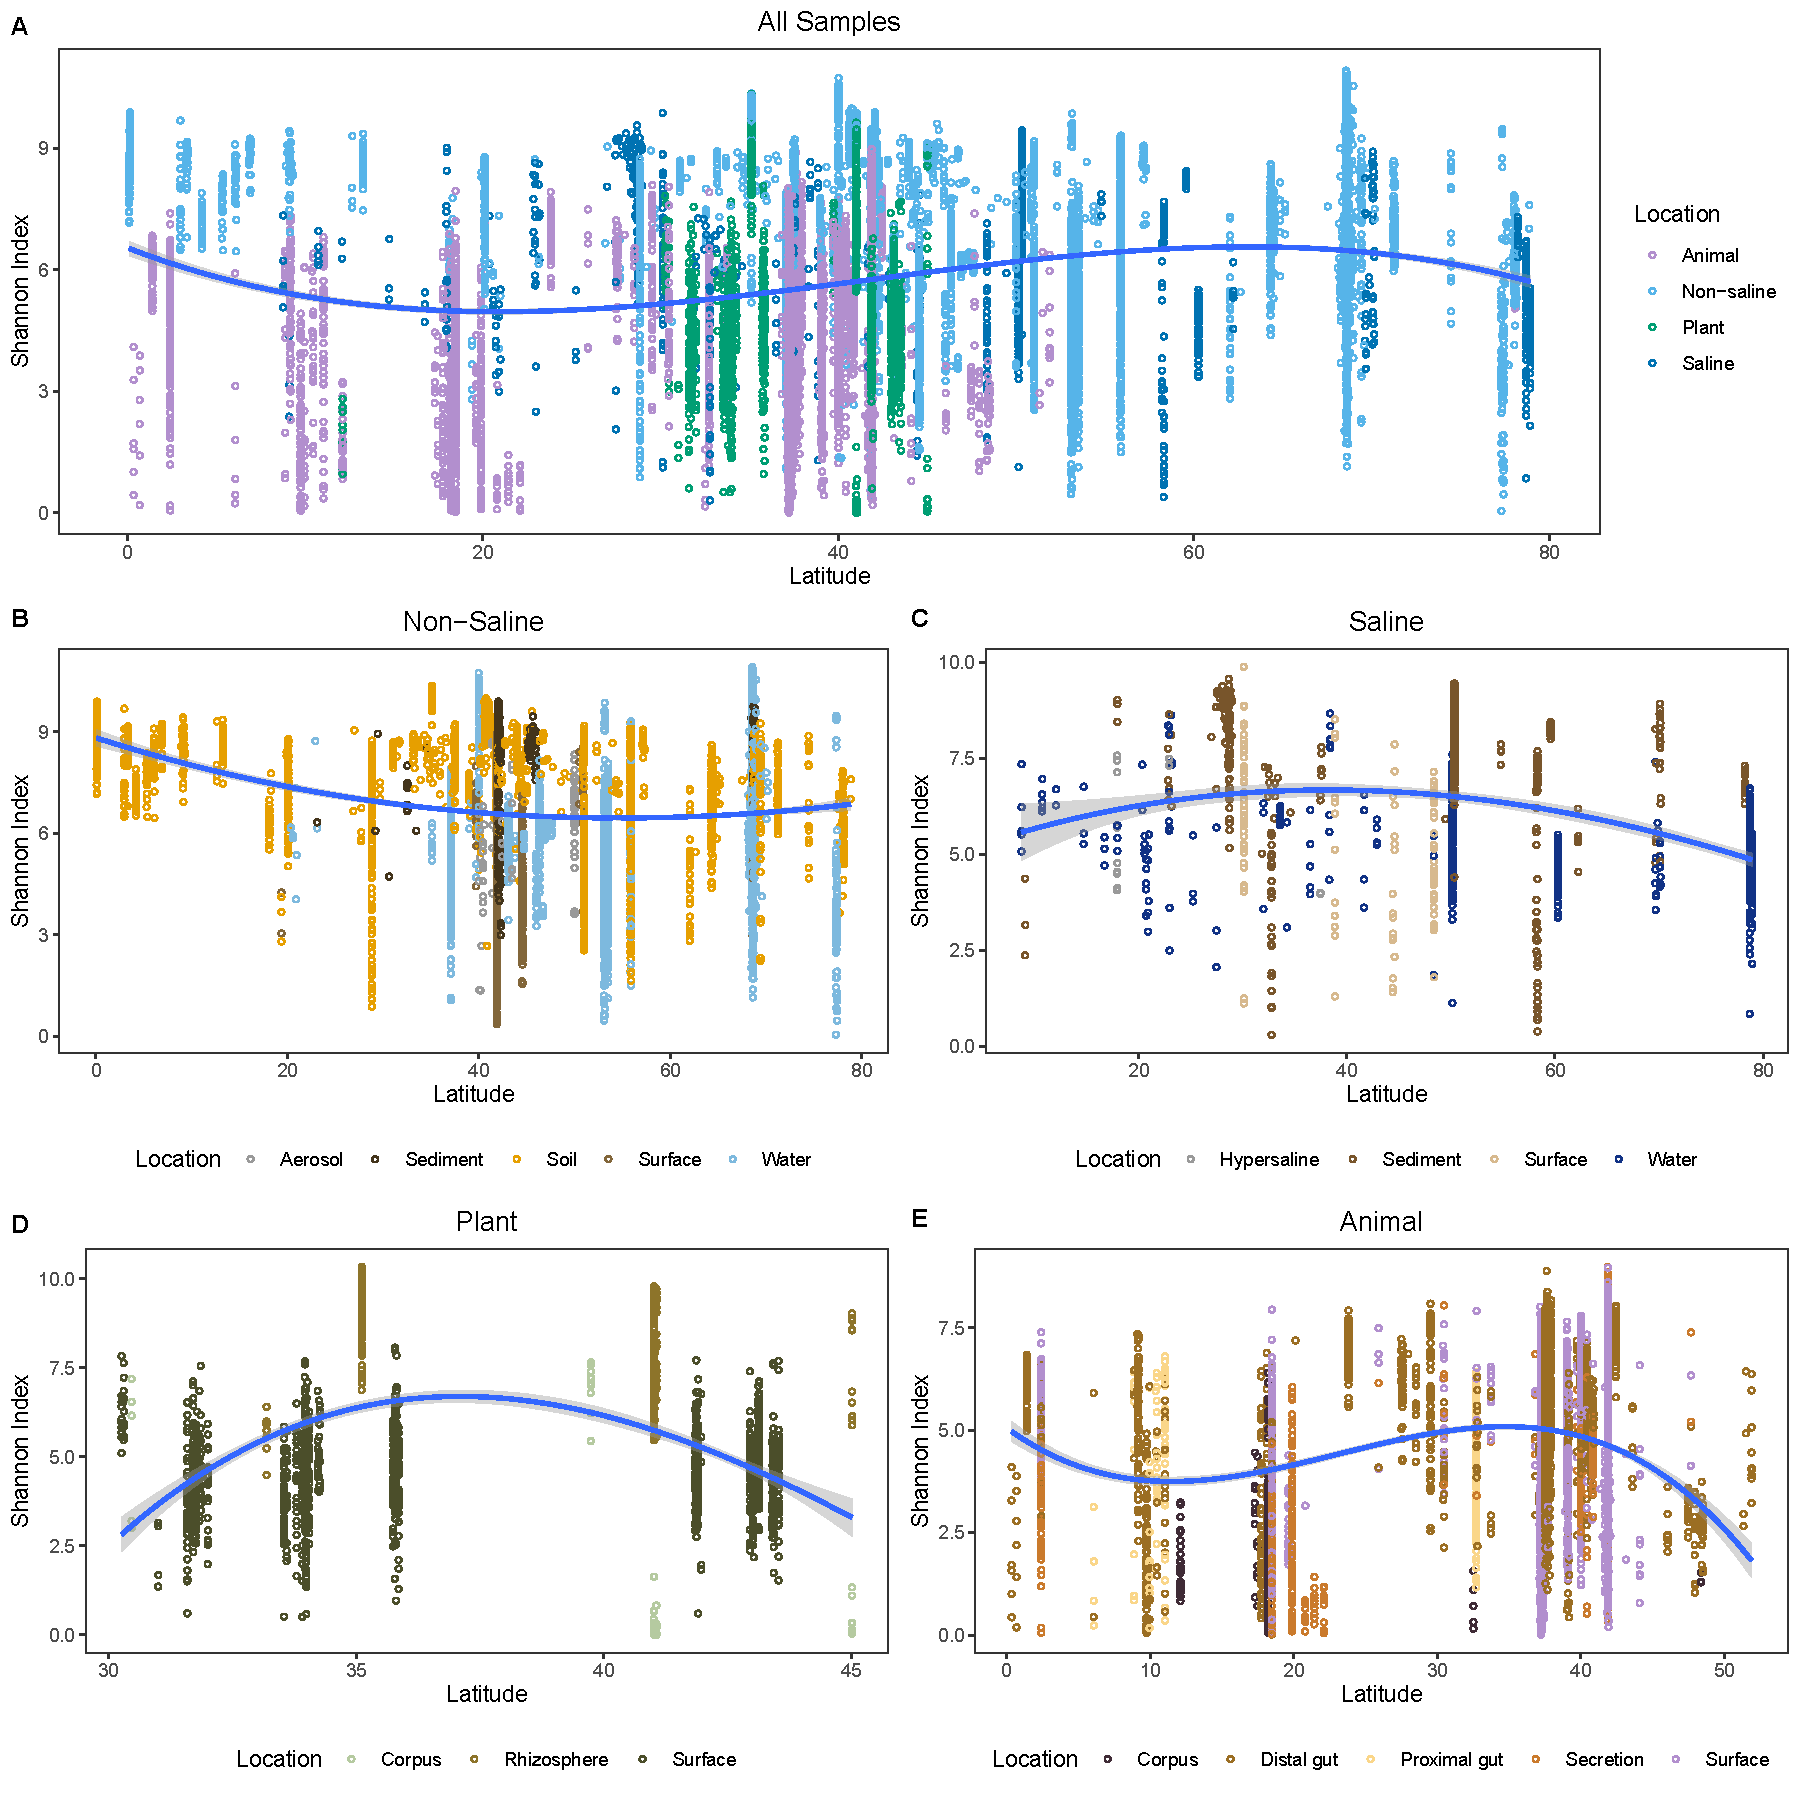
\includegraphics[scale=0.33]{./Figures/Shan_lati_empo2}
    \caption{\textbf{The relationship between Shannon index and latitude.} A: Trend of Shannon index with latitude for samples in the whole dataset. B: Trend of Shannon index with latitude for non-saline samples. C: Trend of Shannon index with latitude for saline samples. D: Trend of Shannon index with latitude for plant samples. E: Trend of Shannon index with latitude for animal samples.}
    \label{fig:Shan_lati}
\end{figure}

\begin{figure}[H]
    \centering
    \includegraphics[scale=0.33]{./Figures/OO_lati_empo3}
    \caption{\textbf{The relationship between observed OTUs and latitude.} A: Trend of observed OTUs with latitude for soil samples. B: Trend of observed OTUs with latitude for non-saline water (water and sediment) samples. C: Trend of observed OTUs with latitude for saline water (water and sediment) samples. D: Trend of observed OTUs with latitude for non-saline sediment samples. E: Trend of observed OTUs with latitude for non-saline surface samples. F: Trend of observed OTUs with latitude for non-saline water samples. G: Trend of observed OTUs with latitude for saline sediment samples. H: Trend of observed OTUs with latitude for saline surface samples. I: Trend of observed OTUs with latitude for saline water samples. J: Trend of observed OTUs with latitude for animal surface samples. K: Trend of observed OTUs with latitude for plant surface samples. L: Trend of observed OTUs with latitude for plant rhizosphere samples.}
    \label{fig:OO_lati3}
\end{figure}


\begin{figure}[H]
    \centering
    \includegraphics[scale=0.33]{./Figures/Shan_lati_empo3}
    \caption{\textbf{The relationship between Shannon index and latitude.} A: Trend of Shannon index with latitude for soil samples. B: Trend of Shannon index with latitude for non-saline water (water and sediment) samples. C: Trend of Shannon index with latitude for saline water (water and sediment) samples. D: Trend of Shannon index with latitude for non-saline sediment samples. E: Trend of Shannon index with latitude for non-saline surface samples. F: Trend of Shannon index with latitude for non-saline water samples. G: Trend of Shannon index with latitude for saline sediment samples. H: Trend of Shannon index with latitude for saline surface samples. I: Trend of Shannon index with latitude for saline water samples. J: Trend of Shannon index with latitude for animal surface samples. K: Trend of Shannon index with latitude for plant surface samples. L: Trend of Shannon index with latitude for plant rhizosphere samples.}
    \label{fig:Shan_lati3}
\end{figure}


\subsection{The relationships between alpha diversity and environmental variables}

\begin{figure}[H]
    \centering
    \includegraphics[scale=0.15]{./Figures/PairsPlot}
    \caption{\textbf{The relationship between alpha diversity indices, temperature, pH and latitude.} A: The relationship between Chao1 index, temperature, pH and latitude. B: The relationship between observed OTUs, temperature, pH and latitude. C: The relationship between Shannon index, temperature, pH and latitude..}
    \label{fig:Pairs}
\end{figure}

\begin{figure}[H]
    \centering
    \includegraphics[scale=0.33]{./Figures/OO_LM_PM_simpleTpL}
    \caption{\textbf{Linear and polynomial regression models of Observed OTUs with a single environmental variable.} A: Linear model of Observed OTUs versus temperature. B: Linear model of Observed OTUs versus pH. C: Linear model of Observed OTUs versus latitude. D: Polynomial regression model of Observed OTUs versus temperature. E: Polynomial regression model of Observed OTUs versus pH. F: Polynomial regression model of Observed OTUs versus latitude.}
    \label{fig:OO_simpleTpL}
\end{figure}

\begin{figure}[H]
    \centering
    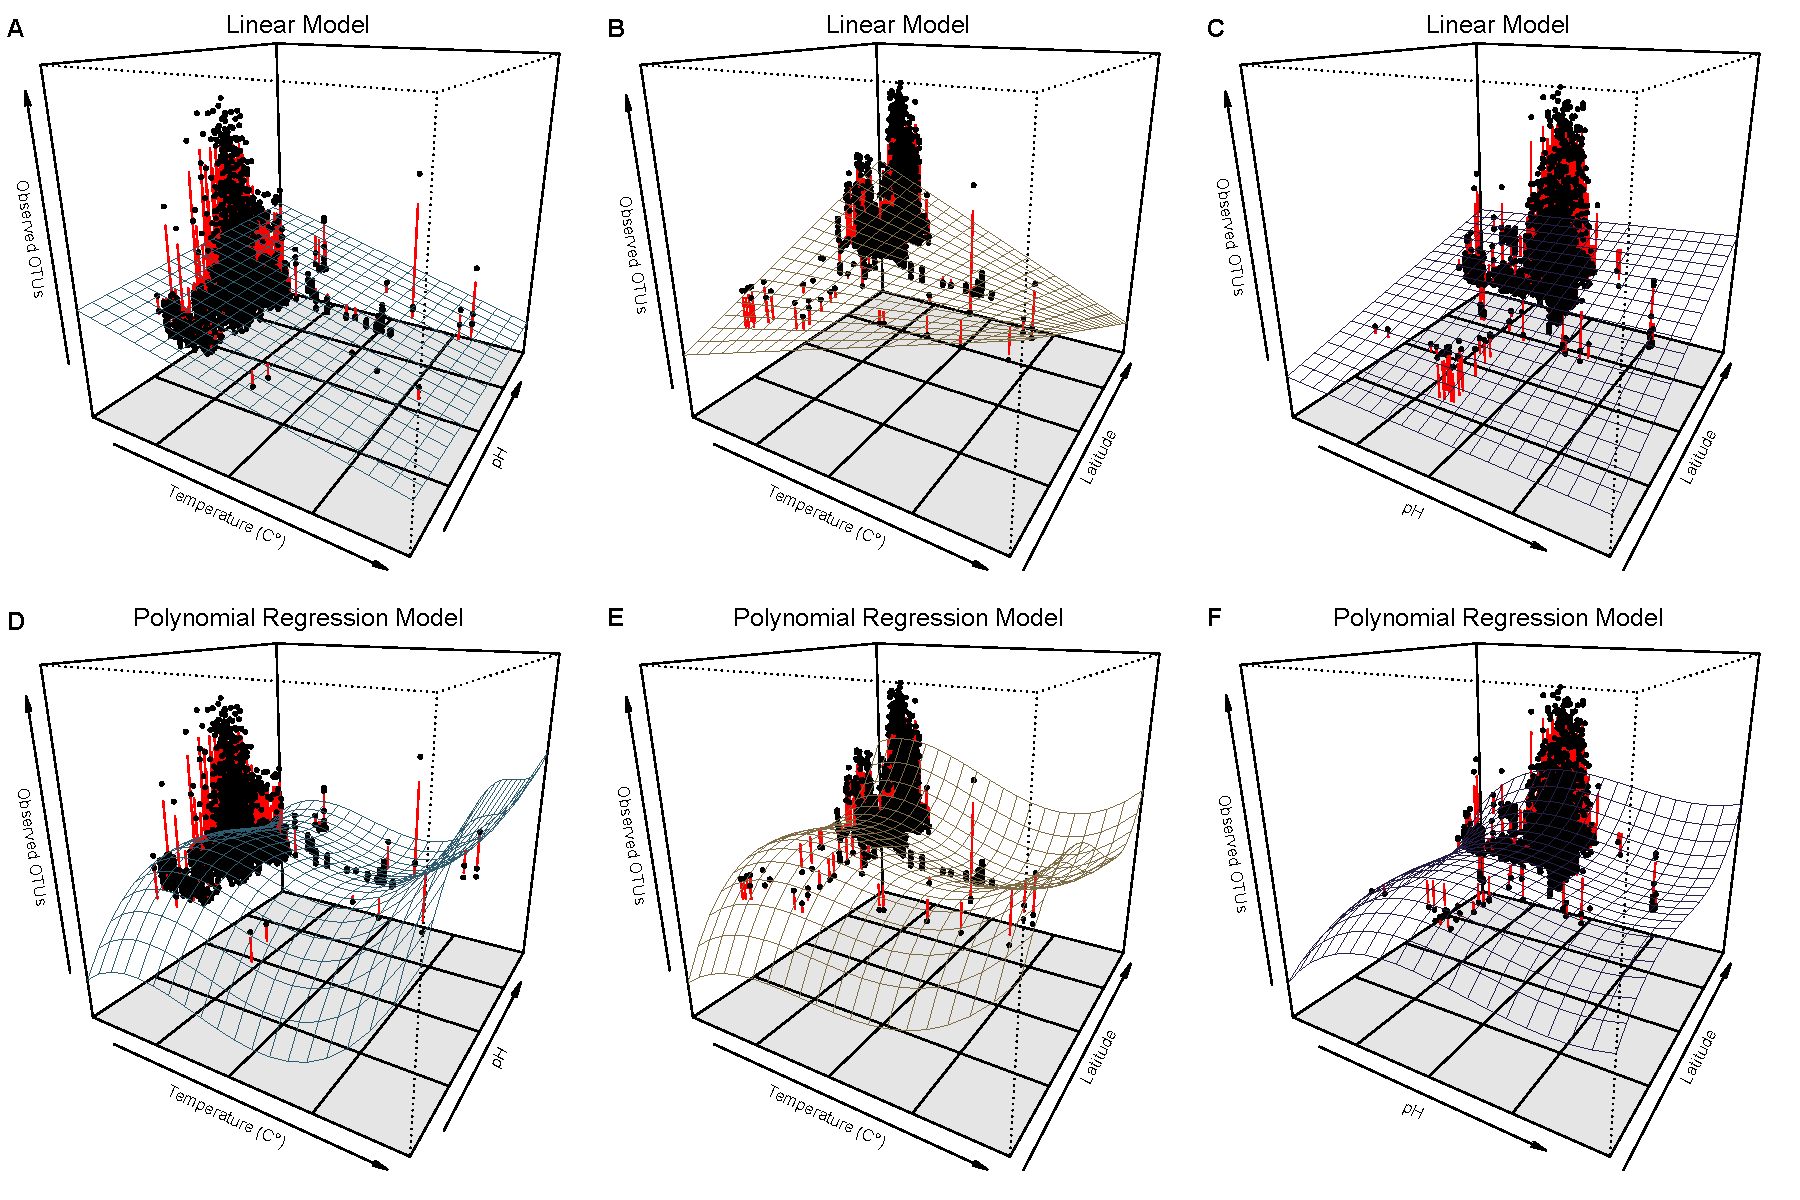
\includegraphics[scale=0.33]{./Figures/OO_LM_PM_all_2EVs_3D}
    \caption{\textbf{Linear and polynomial regression models of Observed OTUs with two environmental variables.} A: Linear model of Observed OTUs versus temperature and pH. B: Linear model of Observed OTUs versus temperature and latitude. C: Linear model of Observed OTUs versus pH and latitude. D: Polynomial regression model of Observed OTUs versus temperature and pH. E: Polynomial regression model of Observed OTUs versus temperature and latitude. F: Polynomial regression model of Observed OTUs versus pH and latitude.}
    \label{fig:OO_2EVs}
\end{figure}

\begin{figure}[H]
    \centering
    \includegraphics[scale=0.33]{./Figures/Shan_LM_PM_simpleTpL}
    \caption{\textbf{Linear and polynomial regression models of Shannon index with a single environmental variable.} A: Linear model of Shannon index versus temperature. B: Linear model of Shannon index versus pH. C: Linear model of Shannon index versus latitude. D: Polynomial regression model of Shannon index versus temperature. E: Polynomial regression model of Shannon index versus pH. F: Polynomial regression model of Shannon index versus latitude.}
    \label{fig:Shan_simpleTpL}
\end{figure}

\begin{figure}[H]
    \centering
    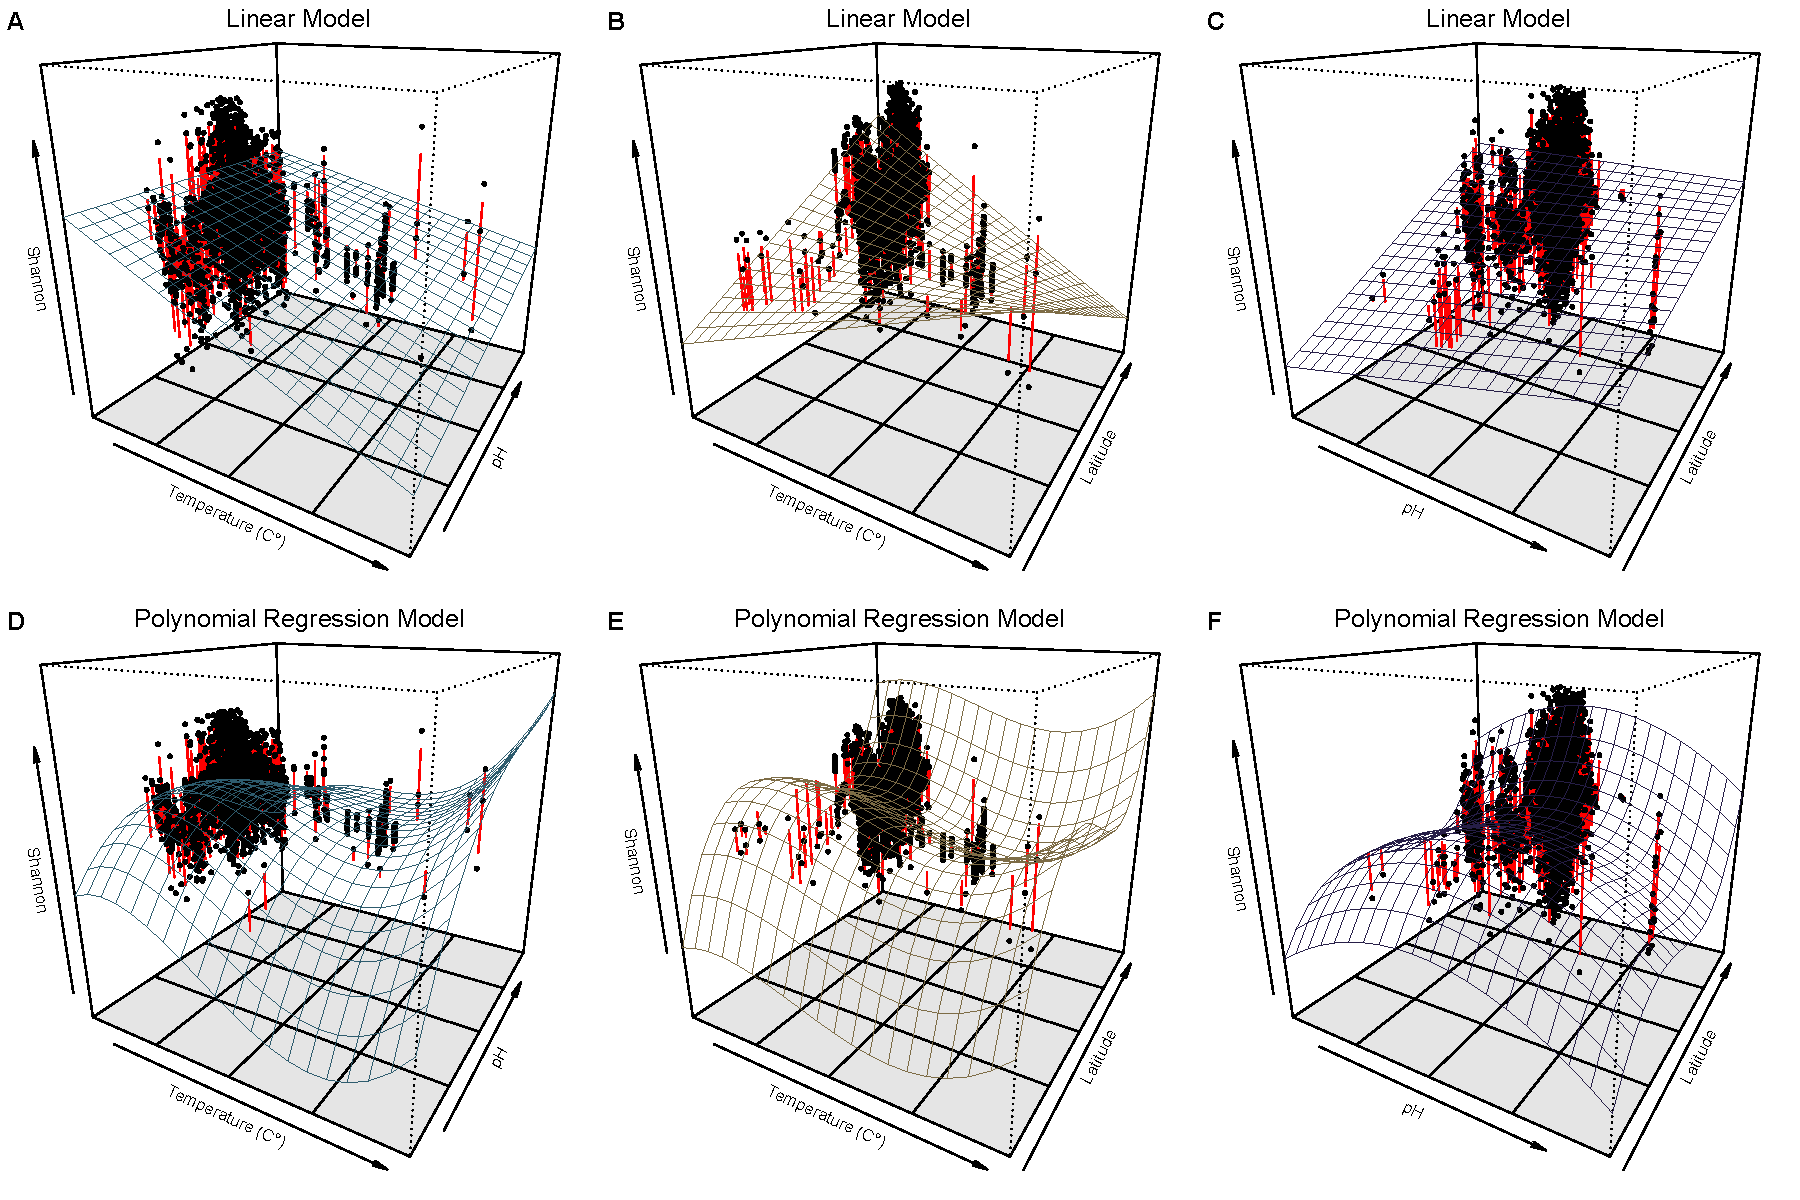
\includegraphics[scale=0.33]{./Figures/Shan_LM_PM_all_2EVs_3D}
    \caption{\textbf{Linear and polynomial regression models of Shannon index with two environmental variables.} A: Linear model of Shannon index versus temperature and pH. B: Linear model of Shannon index versus temperature and latitude. C: Linear model of Shannon index versus pH and latitude. D: Polynomial regression model of Shannon index versus temperature and pH. E: Polynomial regression model of Shannon index versus temperature and latitude. F: Polynomial regression model of Shannon index versus pH and latitude.}
    \label{fig:Shan_2EVs}
\end{figure}

\begin{table}[H]
    \caption{R-square of the EMPO3 models between Chao1 index, observed OTUs and Shannon index and environmental variables.}
    \centering
    \begin{tabular}{ |m{1cm}<{\centering}|m{1.3cm}<{\centering}|m{1.3cm}<{\centering}|m{1.3cm}<{\centering}|m{1.3cm}<{\centering}|m{1.3cm}<{\centering}|m{1.3cm}<{\centering}|m{1.3cm}<{\centering}|m{1.3cm}<{\centering}|m{1.3cm}<{\centering}|} 
    \hline
     $R^{2}$ (NS-Water) & Chao1 (LM) & Chao1 (PM) & Chao1 (RF) & Shannon (LM) & Shannon (PM) & Shannon (RF) & OTUs (LM) & OTUs (PM) & OTUs (RF) \\
     \hline
    T*p*L & 0.1781 & 0.1957 & 0.3979 & 0.2236 & 0.2355 & 0.322 & 0.1665 & 0.1829 & 0.3909 \\
    T*p & NULL & 0.1027 & 0.14 & 0.01416 & 0.1145 & 0.1534 & NULL & 0.09218 & 0.1284 \\
    T*L & 0.1458 & 0.1663 & 0.4269 & 0.2064 & 0.2165 & 0.3233 & 0.1363 & 0.1544 & 0.4304 \\
    p*L & NULL & 0.1344 & 0.4308 & 0.1962 & 0.2064 & 0.3186 & NULL & 0.1233 & 0.4149 \\
    T & 0.003247 & 0.06321 & 0.0186 & 0.0103 & 0.0522 & NULL & 0.004906 & 0.05587 & 0.0116 \\
    p & NULL & 0.06568 & 0.0994 & 0.003669 & 0.09646 & 0.1128 & NULL & 0.06064 & 0.0837 \\
    L & 0.1295 & 0.1327 & 0.4653 & 0.1854 & 0.1961 & 0.3463 & 0.116 & 0.1206 & 0.4609 \\
    \hline
    \hline
     $R^{2}$ (NS-Surf) & Chao1 (LM) & Chao1 (PM) & Chao1 (RF) & Shannon (LM) & Shannon (PM) & Shannon (RF) & OTUs (LM) & OTUs (PM) & OTUs (RF) \\
     \hline
    T*p*L & 0.6096 & 0.6594 & 0.6567 & 0.4957 & 0.5505 & 0.4803 & 0.5749 & 0.6241 & 0.6213 \\
    T*p & 0.4078 & 0.4895 & 0.6621 & 0.273 & 0.2916 & 0.4764 & 0.3603 & 0.4297 & 0.6243 \\
    T*L & NULL & 0.6011 & 0.6373 & NULL & 0.4443 & 0.463 & NULL & 0.5543 & 0.5965 \\
    p*L & 0.2897 & 0.558 & 0.642 & 0.1716 & 0.393 & 0.4681 & 0.2448 & 0.5036 & 0.6008 \\
    T & 0.2403 & 0.4724 & 0.6525 & 0.1373 & 0.2693 & 0.4696 & 0.205 & 0.4216 & 0.6164 \\
    p & 0.038 & 0.3264 & 0.6354 & 0.03825 & 0.1939 & 0.4225 & 0.03848 & 0.276 & 0.5914 \\
    L & NULL & 0.285 & 0.2741 & NULL & 0.2714 & 0.2542 & NULL & 0.2773 & 0.2656 \\
    \hline
    \hline
     $R^{2}$ (S-Sedi) & Chao1 (LM) & Chao1 (PM) & Chao1 (RF) & Shannon (LM) & Shannon (PM) & Shannon (RF) & OTUs (LM) & OTUs (PM) & OTUs (RF) \\
     \hline
    T*p*L & 0.5044 & 0.5044 & 0.4741 & NULL & NULL & 0.4035 & 0.578 & 0.578 & 0.5295 \\
    T*p & NULL & 0.4832 & 0.4342 & NULL & NULL & 0.3925 & NULL & 0.5499 & 0.5121 \\
    T*L & NULL & 0.4758 & 0.4672 & NULL & NULL & 0.3988 & NULL & 0.5554 & 0.5355 \\
    p*L & 0.5016 & 0.5018 & 0.4709 & 0.4109 & NULL & 0.3988 & 0.5717 & 0.5795 & 0.5416 \\
    T & 0.01735 & 0.4322 & 0.4677 & NULL & 0.1402 & 0.3899 & 0.01459 & 0.5115 & 0.5303 \\
    p & NULL & 0.09837 & 0.4275 & NULL & 0.1067 & 0.3854 & NULL & 0.1161 & 0.4941 \\
    L & 0.449 & 0.4559 & 0.447 & 0.3903 & 0.4102 & 0.4007 & 0.5302 & 0.545 & 0.5301 \\
    \hline
    \end{tabular}    
    \label{tab:EMPO3models}
\end{table}

\begin{table}[H]
    \caption{R-square of the local samples models between Chao1 index, observed OTUs and Shannon index and environmental variables. Local 1, 2 and 3 are Yellowstone National Park, Großer Stechlinsee and Toolik Lake respectively.}
    \centering
    \begin{tabular}{ |m{1.3cm}<{\centering}|m{1.2cm}<{\centering}|m{1.2cm}<{\centering}|m{1.2cm}<{\centering}|m{1.4cm}<{\centering}|m{1.4cm}<{\centering}|m{1.4cm}<{\centering}|m{1.3cm}<{\centering}|m{1.3cm}<{\centering}|m{1.2cm}<{\centering}|} 
    \hline
     $R^{2}$ & Chao1 (LM) & Chao1 (PM) & Chao1 (RF) & Shannon (LM) & Shannon (PM) & Shannon (RF) & OTUs (LM) & OTUs (PM) & OTUs (RF) \\
     \hline
    Local 1 T*p & 0.4719 & 0.4918 & 0.6588 & 0.2912 & 0.3152 & 0.4806 & 0.412 & 0.433 & 0.6205 \\
    Local 2 T*p & NULL & NULL & NULL & 0.04069 & 0.04874 & NULL & 0.009332 & 0.0143 & NULL \\
    Local 3 T*p & 0.05701 & 0.08249 & 0.0461 & 0.04255 & 0.05284 & 0.0098 & 0.0594 & 0.08191 & 0.0555 \\
    Local 1 T & 0.2438 & 0.473 & 0.6529 & 0.1433 & 0.267 & 0.4715 & 0.2093 & 0.04204 & 0.6159 \\
    Local 2 T & NULL & 0.003542 & NULL & 0.009679 & 0.009679 & NULL & 0.001895 & 0.003983 & NULL \\
    Local 3 T & 0.01907 & 0.06512 & 0.0185 & 0.03076 & 0.04849 & NULL & 0.0247 & 0.0647 & 0.0272 \\
    Local 1 p & 0.2981 & 0.4996 & 0.6343 & 0.1678 & 0.289 & 0.4266 & 0.2529 & 0.4368 & 0.5872 \\
    Local 2 p & NULL & NULL & NULL & 0.03141 & 0.03629 & NULL & 0.007482 & 0.01022 & NULL \\
    Local 3 p & NULL & 0.00248 & NULL & NULL & NULL & NULL & NULL & 0.001819 & NULL \\
    \hline
    \end{tabular}    
    \label{tab:localmodels}
\end{table}

\end{document}